\documentclass[tikz,border=8pt]{standalone}
% Shared look for every TikZ diagram. Load with \input{../../tools/tikz-style.tex}
\usepackage[T1]{fontenc}
\usepackage{lmodern}
\renewcommand{\sfdefault}{lmr}  % diagrams use the same serif as the text
\usetikzlibrary{arrows.meta, positioning, shapes.geometric, calc, fit, backgrounds}
\definecolor{cblue}{HTML}{4C78A8}
\definecolor{corange}{HTML}{F58518}
\definecolor{cgreen}{HTML}{54A24B}
\definecolor{cred}{HTML}{E45756}
\definecolor{cpurple}{HTML}{B279A2}
\definecolor{cgrey}{HTML}{6B6B6B}
\tikzset{
  every picture/.style={font=\sffamily, line width=1.2pt},
  box/.style={draw=#1, fill=#1!12, rounded corners=4pt, align=center, inner sep=7pt, minimum height=1.1cm},
  box/.default=cgrey,
  arrow/.style={-{Stealth[length=3mm]}, draw=cgrey, line width=1.4pt},
  title/.style={font=\sffamily\bfseries\Large},
  note/.style={font=\sffamily\small, text=cgrey, align=center},
}
\AtBeginDocument{\hyphenpenalty=10000 \exhyphenpenalty=10000}

\begin{document}
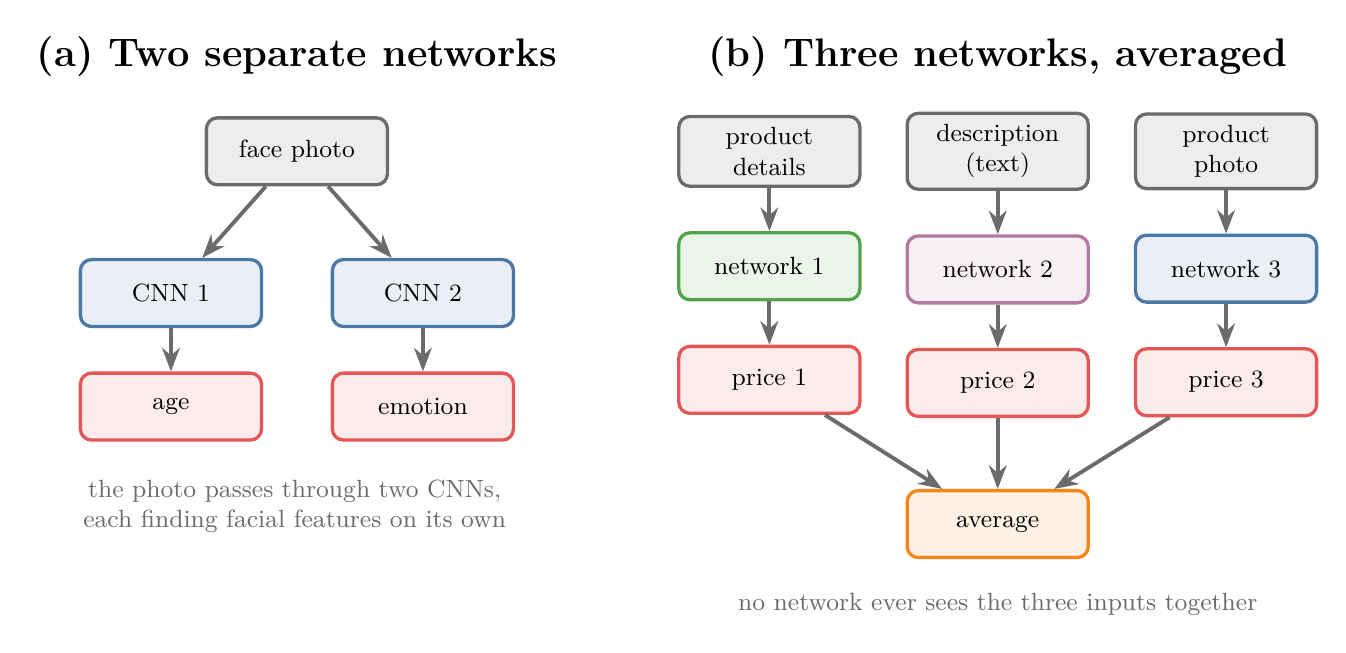
\begin{tikzpicture}[b/.style={box=#1, minimum width=2.3cm, minimum height=0.85cm, inner sep=4pt, font=\sffamily\small}, node distance=0.55cm]
  % (a) two separate networks for two outputs
  \begin{scope}
    \node[title] at (1.6, 1.2) {(a) Two separate networks};
    \node[b=cgrey] (f) at (1.6, 0) {face photo};
    \node[b=cblue] (c1) at (0, -1.8) {CNN 1};
    \node[b=cblue] (c2) at (3.2, -1.8) {CNN 2};
    \node[b=cred, below=of c1] (age) {age};
    \node[b=cred, below=of c2] (emo) {emotion};
    \draw[arrow] (f) -- (c1); \draw[arrow] (f) -- (c2); \draw[arrow] (c1) -- (age); \draw[arrow] (c2) -- (emo);
    \node[note, below=0.35cm of age.south east, xshift=0.4cm] {the photo passes through two CNNs,\\each finding facial features on its own};
  \end{scope}
  % (b) three networks, prices averaged
  \begin{scope}[xshift=7.6cm]
    \node[title] at (2.9, 1.2) {(b) Three networks, averaged};
    \node[b=cgrey] (t) at (0, 0) {product\\details};
    \node[b=cgrey] (x) at (2.9, 0) {description\\(text)};
    \node[b=cgrey] (im) at (5.8, 0) {product\\photo};
    \node[b=cgreen, below=of t] (td) {network 1};
    \node[b=cpurple, below=of x] (xr) {network 2};
    \node[b=cblue, below=of im] (ic) {network 3};
    \node[b=cred, below=of td] (p1) {price 1};
    \node[b=cred, below=of xr] (p2) {price 2};
    \node[b=cred, below=of ic] (p3) {price 3};
    \node[b=corange, below=0.9cm of p2] (avg) {average};
    \foreach \a/\c in {t/td, x/xr, im/ic, td/p1, xr/p2, ic/p3, p1/avg, p2/avg, p3/avg} \draw[arrow] (\a) -- (\c);
    \node[note, below=0.3cm of avg] {no network ever sees the three inputs together};
  \end{scope}
\end{tikzpicture}
\end{document}
